 \documentclass{article}
\usepackage{tikz}
\usetikzlibrary{positioning, automata}
\usepackage{fancyhdr}
\usepackage{extramarks}
\usepackage[plain]{algorithm}
\usepackage{algpseudocode}
\usepackage[utf8]{inputenc} 
\usepackage[T1]{fontenc}    
\usepackage{hyperref}       
\usepackage{url}        
\usepackage{booktabs}
\usepackage{pdfpages}
\usepackage{amsfonts}   
\usepackage{nicefrac}       
\usepackage{microtype}      
\usepackage{amsmath}
\usepackage{graphicx}
\usepackage{float}
\usepackage{caption}
\usepackage{ragged2e}
\usepackage{amssymb}
\usepackage{mathtools}
\usepackage{xcolor}
\usepackage[spanish]{babel} % ¡Solo una vez!
\usepackage{array}
\usepackage{multirow}
\usepackage{multicol}
\usepackage{manfnt}
\usepackage{layout}
\usepackage{manfnt}
\usepackage{phaistos}
\usepackage{polynom}
\usepackage[most]{tcolorbox}
\RequirePackage{algorithm}
\RequirePackage{algpseudocode}


\setcounter{page}{0}
%
% Basic Document Settings
%

\topmargin=-0.45in
\evensidemargin=0in
\oddsidemargin=0in
\textwidth=6.5in
\textheight=9.0in
\headsep=0.25in

\linespread{1.1}
%|#*******************************************************************#|
\pagestyle{fancy}
\lhead{Taller}
\chead{\hmwkClass\ : \hmwkTitle}
\rhead{\firstxmark}
\lfoot{\lastxmark}
\cfoot{\thepage}

\renewcommand\headrulewidth{0.4pt}
\renewcommand\footrulewidth{0.4pt}

\setlength\parindent{0pt}

%
% Create Problem Sections
%

\newcommand{\enterProblemHeader}[1]{
    \nobreak\extramarks{}{Problema \arabic{#1} continúa en la siguiente página\ldots}\nobreak{}
    \nobreak\extramarks{Problema \arabic{#1} (continuación}{Problema \arabic{#1} continúa en la siguiente página\ldots}\nobreak{}
}

\newcommand{\exitProblemHeader}[1]{
    \nobreak\extramarks{Problema \arabic{#1} (continuación)}{Problema \arabic{#1} continúa en la siguiente página\ldots}\nobreak{}
    \stepcounter{#1}
    \nobreak\extramarks{Problema \arabic{#1}}{}\nobreak{}
}



\setcounter{secnumdepth}{0}
\newcounter{partCounter}
\newcounter{homeworkProblemCounter}
\setcounter{homeworkProblemCounter}{1}
\nobreak\extramarks{Problema \arabic{homeworkProblemCounter}}{}\nobreak
%margen de una pagina
\newenvironment{changemargin}[2]{%
\begin{list}{}{%
\setlength{\topsep}{0pt}%
\setlength{\leftmargin}{#1}%
\setlength{\rightmargin}{#2}%
\setlength{\listparindent}{\parindent}%
\setlength{\itemindent}{\parindent}%
\setlength{\parsep}{\parskip}%
}%
\item[]}{\end{list}}

%
% Homework Problem Environment
%
% This environment takes an optional argument. When given, it will adjust the
% problem counter. This is useful for when the problems given for your
% assignment aren't sequential. See the last 3 problems of this template for an
% example.
%
\newenvironment{homeworkProblem}[1][-1]{
    \ifnum#1>0
        \setcounter{homeworkProblemCounter}{#1}
    \fi
    \section{Problema \arabic{homeworkProblemCounter}:}
    \setcounter{partCounter}{1}
    \enterProblemHeader{homeworkProblemCounter}
}{
    \exitProblemHeader{homeworkProblemCounter}
}


%|#*******************************************************************#|

\newcommand{\hmwkTitle}{Taller 2}
\newcommand{\hmwkClass}{EDP I}
\newcommand{\hmwkUniversity}{Universidad Nacional de Colombia}
\newcommand{\hmwkAuthorName}{Edgar Santiago Ochoa Quiroga}
\newcommand{\hmwkInstructor}{\empty}

%
% Title Page
%

\title{
    \vspace{2in}
    \textmd{\textbf{\hmwkClass:\ \hmwkTitle}}\\
    \vspace{0.1in}\large{\textit{\hmwkUniversity}}\\
    \vspace{1.5in} \textrm{\hmwkInstructor}
    \vspace{1.5in}
}

\author{\hmwkAuthorName}
\date{}

\renewcommand{\part}[1]{\textbf{\large Part \Alph{partCounter}}\stepcounter{partCounter}\\}
%
%   Nuevos tipos de columna
%
\newcolumntype{C}{>{$}c<{$}}
\newcolumntype{L}{>{$}l<{$}}
\newcolumntype{R}{>{$}r<{$}}
% ---------------------------
%|  Various Helper Commands  |
% ---------------------------

% Useful for algorithms
\newcommand{\alg}[1]{\textsc{\bfseries \footnotesize #1}}

% -For derivatives-
\newcommand{\deriv}[2]{\frac{\mathrm{d #1 }}{\mathrm{d} #2} }

%For derivatives of degree >1
\newcommand{\mderiv}[3]{\frac{\mathrm{d^{#3} #1 }}{\mathrm{d} #2} }

% -For partial derivatives-
\newcommand{\pderiv}[2]{\frac{\partial}{\partial #1} (#2)}

% -Integral dx-
\newcommand{\dx}{\hspace{3pt}\mathrm{d}}

% Alias for the Solution section header
\newcommand{\solution}{\textbf{\\\\\large Solución:\\ \hspace*{5pt}}}

% Probability commands: Expectation, Variance, Covariance, Bias
\newcommand{\E}{\mathrm{E}}
\newcommand{\Var}{\mathrm{Var}}
\newcommand{\Cov}{\mathrm{Cov}}
\newcommand{\Bias}{\mathrm{Bias}}


%TcolorBox

% Definir colores y la tcolorbox de la solución
\definecolor{myDColor}{HTML}{101010} 

\definecolor{myLColor}{RGB}{153,204,255} 

\definecolor{LinkColor}{HTML}{9669d9} 


\newtcolorbox{solucion}[1][]{%
    enhanced,
    skin first=enhanced,
    skin middle=enhanced,
    skin last=enhanced,
    before upper={\parindent15pt},
    breakable,
    boxrule = 0pt,
    frame hidden,
    borderline west = {4pt}{0pt}{myDColor},
    colback = myLColor!5,
    coltitle = myLColor!5,
    sharp corners,
    rounded corners = southeast,
    arc is angular,
    arc = 3mm,
    attach boxed title to top left,
    boxed title style = {%
        enhanced,
        colback = myDColor,
        colframe = myDColor,
        top = 0pt,
        bottom = 0pt,
        sharp corners,
        rounded corners = northeast,
        arc is angular,
        arc = 2mm,
        rightrule = 0pt,
        bottomrule = 0pt,
        toprule = 0pt,
    },
    title = {\bfseries\large Solución:}, 
    overlay unbroken={%
        \node[anchor=west, color=black!70] at (title.east) {#1};
        \path[fill = tcbcolback!80!black] 
            ([yshift = 3mm]interior.south east) -- ++(-0.4,-0.1) -- ++(0.1,-0.2);
    },
    overlay first = {%
        \node[anchor=west, color=black!70] at (title.east) {#1};
        \path[fill = tcbcolback!80!black] 
            ([yshift = 3mm]interior.south east) -- ++(-0.4,-0.1) -- ++(0.1,-0.2);
    },
    overlay middle={%
        \path[fill = tcbcolback!80!black] 
            ([yshift = -3mm]interior.north east) -- ++(-0.4,0.1) -- ++(0.1,0.2);
        \path[fill = tcbcolback!80!black] 
            ([yshift = 3mm]interior.south east) -- ++(-0.4,-0.1) -- ++(0.1,-0.2);
    },
    overlay last={%
        \path[fill = tcbcolback!80!black] 
            ([yshift = -3mm]interior.north east) -- ++(-0.4,0.1) -- ++(0.1,0.2);
        \path[fill = tcbcolback!80!black] 
            ([yshift = 3mm]interior.south east) -- ++(-0.4,-0.1) -- ++(0.1,-0.2);
    },
    extras middle and last = { rounded corners = northeast }
}
\newcommand{\qed}{\hfill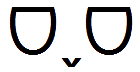
\includegraphics[height=2ex]{Demo_face-removebg-preview .png}}
\usepackage{amsmath}
\usepackage{geometry}
\usepackage{tikz}
\usepackage{float}
\usepackage{graphics}

\tikzset{every picture/.style={line width=0.75pt}} %set default line width to 0.75pt        

\begin{document}
\maketitle
\thispagestyle{empty}
\newpage 
\begin{homeworkProblem}
    Clasifique las siguientes ecuaciones según su tipo y llévelas a su forma canónica
    \begin{itemize}
        \item [i)]$4u_{xx}+12u_{xy}+5u_{yy}=6u_x-u_y$
        \begin{solucion}
         Notemos que los coeficientes que acompañan a las derivadas de segundo orden son $a=4,b=6$ y $c=5$ de esta forma el discriminante es:
         $$\delta(x,y)=6^2-4\cdot5=16>0$$
         Así concluimos que la ecuación es de tipo \textbf{hiperbólico}. Ahora procedemos a hallar nuestros cambios de variable haciendo uso de las curvas características:
         $$\dfrac{dy}{dx}=\dfrac{6\pm\sqrt{16} }{4}$$
         De esta forma tenemos las siguientes ecuaciones:
         \begin{align*}
             \dfrac{dy}{dx}&=\dfrac{5}{2} &   \dfrac{dy}{dx}&=\dfrac{1}{2} 
             \end{align*}
             y resolviéndolas obtenemos:
             \begin{align*}
                 y&=\dfrac{5}{2}x+c_1 & y&=\dfrac{1}{2}x+c_2
             \end{align*}
             luego si despejamos las constantes:
             \begin{align*}
             c_1&=y-\dfrac{5}{2}x & c_2&=y-\dfrac{1}{2}x    
             \end{align*}
             De esta forma ya podemos definir nuestro cambio de variable que viene dado de igualar $\xi=c_1$ y $\eta=c_2$, es decir:
             \begin{align*}
             \xi&=y-\dfrac{5}{2}x & \eta&=y-\dfrac{1}{2}x    
             \end{align*}
             Ahora procedamos con llevar nuestra EDP a la forma canónica. Si hacemos \\$V(\xi,\eta)=u(x,y)$ determinemos las derivadas necesarias para luego reemplazar en la EDP:
             \begin{align*}
                 u_x&=V_\xi \xi_x+V_\eta \eta_x\\
                &=-\dfrac{5}{2}V_\xi-\dfrac{1}{2}V_\eta\\
                \\
                u_{xx}&=-\dfrac{5}{2}(V_{\xi\xi}\xi_x+V_{\xi\eta}\eta_x)-\dfrac{1}{2}(V_{\eta\eta}\eta_x+V_{\xi\eta}\xi_x)\\
                &=-\dfrac{5}{2}(-\dfrac{5}{2}V_{\xi\xi}-\dfrac{1}{2}V_{\xi\eta})-\dfrac{1}{2}(-\dfrac{1}{2}V_{\eta\eta}-\dfrac{5}{2}V_{\xi\eta})\\
                &=\dfrac{25}{4}V_{\xi\xi}+\dfrac{5}{2}V_{\xi\eta}+\dfrac{1}{4}V_{\eta\eta}\\
                \\
                u_{xy}&=-\dfrac{5}{2}(V_{\xi\xi}\xi_y+V_{\xi\eta}\eta_y)-\dfrac{1}{2}(V_{\eta\eta}\eta_y+V_{\xi\eta}\xi_y)\\
                &=-\dfrac{5}{2}V_{\xi\xi}-\dfrac{5}{2}V_{\xi\eta}-\dfrac{1}{2}V_{\eta\eta}-\dfrac{1}{2}V_{\xi\eta}\\
                &=-\dfrac{5}{2}V_{\xi\xi}-3V_{\xi\eta}-\dfrac{1}{2}V_{\eta\eta}
                \\
                u_y&=V_\xi \xi_y+V_\eta \eta_y\\
                 &=V_\xi+V_\eta\\
                 \\
                u_{yy}&=V_{\xi\xi}\xi_y+V_{\xi\eta}\eta_y+V_{\eta\eta}\eta_y+V_{\xi\eta}\xi_y\\
                &=V_{\xi\xi}+2V_{\xi\eta}+V_{\eta\eta}
             \end{align*}
             Ahora ya con todo esto determinado procedemos reemplazar en las siguientes expresiones
             \begin{align*}
             4u_{xx}+12u_{xy}+5u_{yy}&=25V_{\xi\xi}+10V_{\xi\eta}+V_{\eta\eta}-30V_{\xi\xi}-36V_{\xi\eta}-6V_{\eta\eta}\\&\hspace{5cm}+5V_{\xi\xi}+10V_{\xi\eta}+5V_{\eta\eta} \\
             &=-16V_{\xi\eta}\\
             \\
             6u_x-u_y&=-15V_\xi-3V_\eta-V_\xi-V_\eta\\
             &=-16V_\xi-4V_\eta
             \end{align*}
             Finalmente reemplazando estos valores en la EDP obtenemos que:
             $$-16V_{\xi\eta}=-16V_\xi-4V_\eta$$
             O en una forma mas simplificada esta seria la EDP en su forma canónica:
             $$V_{\xi\eta}=V_\xi+\dfrac{1}{4}V_\eta$$
             \qed
        \end{solucion}
        \item[ii)] $u_{xx}-4u_{xy}+4u_{yy}=4+2u_x$
        \begin{solucion}
            Los coeficientes de la EDP son $a=1, b=-2$ y $c=4$ luego:
            $$\delta(x,y)=4-4=0$$
            Esto quiere decir que la ecuación es de tipo \textbf{parabólico} y por tanto solo tenemos una ecuación característica dada por:
            $$\dfrac{dy}{dx}=-2$$
            Si la resolvemos obtenemos que $y=-2x+c$ y despejando la constante tenemos que $c=y+2x$. Así tenemos que si $\xi=c$ entonces $\xi=y+2x$. Ahora estudiemos el jacobiano para proponer un $\eta$ adecuado:
            $$\det\begin{pmatrix}
                \xi_x & \xi_y \\
                \eta_x & \eta_y \\
            \end{pmatrix}=\det\begin{pmatrix}
               2 & 1 \\ 
               \eta_x & \eta_y \\
            \end{pmatrix}=2\eta_y-\eta_x\neq 0$$
            Note que esta condición se cumple si $\eta=y$ así que ese es nuestro cambio de variable adecuado. Ahora si $V(\xi,\eta)=u(x,y)$ procedemos con determinar la derivadas necesarias para reemplazar en la EDP:
            \begin{align*}
                u_x&=V_\xi \xi_x+V_\eta \eta_x\\
                 &=2V_\xi\\
                 \\
                 u_{xx}&=2(V_{\xi\xi}\xi_x+V_{\xi\eta}\eta_x)\\
                 &=4V_{\xi\xi}\\
                 \\
                 u_{xy}&=2(V_{\xi\xi}\xi_y+V_{\xi\eta}\eta_y)\\
                 &=2V_{\xi\xi}+2V_{\xi\eta}\\
                 \\
                 u_y&=V_\xi \xi_y+V_\eta \eta_y\\
                 &=V_\xi+V_\eta \\
                 \\
                  u_{yy}&=V_{\xi\xi}\xi_y+V_{\xi\eta}\eta_y+V_{\eta\eta}\eta_y+V_{\xi\eta}\xi_y\\
                &=V_{\xi\xi}+2V_{\xi\eta}+V_{\eta\eta}
            \end{align*}
            Ahora procedemos a reemplazar en las siguientes expresiones:
            \begin{align*}
                u_{xx}-4u_{xy}+4u_{yy}&=4V_{\xi\xi}-8V_{\xi\xi}-8V_{\xi\eta}+4V_{\xi\xi}+8V_{\xi\eta}+4V_{\eta\eta}\\
                &=4V_{\eta\eta}\\
                4+2u_x&=4+4V_\xi
            \end{align*}
            Finalmente reemplazando en la EDP obtenemos que:
            $$4V_{\eta\eta}=4+4V_\xi$$
            y simplificando un poco llegamos a que la forma canónica de la EDP es:
            $$V_{\eta\eta}=1+V_\xi$$
            \qed
        \end{solucion}
        \item [iii)]$(1+x^2)^2\partial^2_xu-(1+y^2)^2\partial^2_yu=0$
        \begin{solucion}
            De la EDP sabemos que los coeficientes son $a=(1+x^2)^2, b=0$ y $c=-(1+y^2)^2.$ Luego tenemos que:
            $$\delta(x,y)=(1+x^2)^2(1+y^2)^2>0$$
            De este modo la ecuación es de tipo \textbf{hiperbólico} Así que  podemos proceder hallando las características dadas por:
            $$ \dfrac{dy}{dx}=\dfrac{\pm\sqrt{(1+x^2)^2(1+y^2)^2}}{(1+x^2)^2}$$
            Así tenemos las siguientes ecuaciones:
            \begin{align*}
                \dfrac{dy}{dx}&=\dfrac{1+y^2}{1+x^2} &  \dfrac{dy}{dx}&=-\dfrac{1+y^2}{1+x^2}\\
                \arctan y&=\arctan x +c_1 & \arctan y&=-\arctan x +c_2
            \end{align*}
            De esta manera si tomamos $\xi=c_1$ y $\eta=c_2$ tenemos que nuestros cambios de variable son:
            \begin{align*}
                \xi&=\arctan y-\arctan x & \eta&=\arctan y+\arctan x
            \end{align*}
            Ahora si consideramos $V(\xi,\eta)=u(x,y)$ realicemos las derivadas respectivas para posteriormente reemplazar:
            \begin{align*}
                u_x&=V_\xi \xi_x+V_\eta \eta_x\\
                &=-\dfrac{1}{1+x^2}V_\xi+\dfrac{1}{1+x^2}V_\eta\\
                \\
                u_{xx}&=\dfrac{2x}{(1+x^2)^2}V_\xi-\dfrac{1}{1+x^2}V_{\xi\xi}\xi_x-\dfrac{1}{1+x^2}V_{\xi\eta}\eta_x-\dfrac{2x}{(1+x^2)^2}V_\eta\\
                &\hspace{5cm}+\dfrac{1}{1+x^2}V_{\eta\eta}\eta_x+\dfrac{1}{1+x^2}V_{\xi\eta}\xi_x\\
                &=\dfrac{2x}{(1+x^2)^2}V_\xi+\dfrac{1}{(1+x^2)^2}V_{\xi\xi}-\dfrac{1}{(1+x^2)^2}V_{\xi\eta}-\dfrac{2x}{(1+x^2)^2}V_\eta\\
                &\hspace{5cm}+\dfrac{1}{(1+x^2)^2}V_{\eta\eta}-\dfrac{1}{(1+x^2)^2}V_{\xi\eta}\\
                &=\dfrac{1}{(1+x^2)^2}(2xV_\xi+V_{\xi\xi}-2V_{\xi\eta}-2xV_\eta+V_{\eta\eta})\\
                \\
                u_y&=V_\xi \xi_y+V_\eta \eta_y\\
                &=\dfrac{1}{1+y^2}V_\xi+\dfrac{1}{1+y^2}V_\eta\\
                &=\dfrac{1}{1+y^2}(V_\xi+V_\eta)\\
                \\
                u_{yy}&=-\dfrac{2y}{(1+y^2)^2}(V_\xi+V_\eta)+\dfrac{1}{1+y^2}(V_{\xi\xi}\xi_y+V_{\xi\eta}\eta_y+V_{\xi\eta}\xi_y+V_{\eta\eta}\eta_y)\\
                &=\dfrac{1}{(1+y^2)^2}(-2yV_\xi-2yV_\eta)+\dfrac{1}{(1+y^2)^2}(V_{\xi\xi}+2V_{\xi\eta}+V_{\eta\eta})\\
                &=\dfrac{1}{(1+y^2)^2}(-2yV_\xi-2yV_\eta+V_{\xi\xi}+2V_{\xi\eta}+V_{\eta\eta})
            \end{align*}
            Y reemplazando en la expresión obtenemos que:
            \begin{align*}
                (1+x^2)^2\partial^2_xu-(1+y^2)^2\partial^2_yu&=2xV_\xi+V_{\xi\xi}-2V_{\xi\eta}-2xV_\eta+V_{\eta\eta}\\&+2yV_\xi+2yV_\eta-V_{\xi\xi}-2V_{\xi\eta}-V_{\eta\eta}\\
                &=(2x+2y)V_\xi+(2y-2x)V_\eta-4V_{\xi\eta}
            \end{align*}
            Así obtenemos que la EDP seria:
            $$V_{\xi\eta}=\dfrac{1}{2}[(y+x)V_\xi+(y-x)V_\eta]$$
            Note que aun no hemos terminado ya que debemos quedarnos solo con funciones de $\xi$ y $\eta$ pero notemos que $y=\tan\left(\dfrac{\xi+\eta}{2}\right)$ y $x=\tan\left(\dfrac{\eta-\xi}{2}\right)$ El despejar esta asegurado aquí ya que el jacobiano siempre es distinto de 0 en este caso:
            \begin{align*}
               \det\begin{pmatrix}
                \xi_x &\xi_y\\
                \eta_x &\eta_y
            \end{pmatrix}=\det\begin{pmatrix}
             \dfrac{-1}{x^2+1}&\dfrac{1}{y^2+1}\\
             \dfrac{1}{x^2+1}&\dfrac{1}{y^2+1}
            \end{pmatrix}&=\dfrac{-1}{(x^2+1)(y^2+1)}-\dfrac{1}{(x^2+1)(y^2+1)} \\
            &=\dfrac{-2}{(x^2+1)(y^2+1)}\neq0
            \end{align*}
            Así podemos concluir que la forma canónica de la EDP es:
            $$V_{\xi\eta}=\dfrac{1}{2}\left[\left(\tan\left(\dfrac{\xi+\eta}{2}\right)+\tan\left(\dfrac{\eta-\xi}{2}\right)\right)V_\xi+\left(\tan\left(\dfrac{\xi+\eta}{2}\right)-\tan\left(\dfrac{\eta-\xi}{2}\right)\right)V_\eta\right]$$
            \qed
        \end{solucion}
    \end{itemize}
\end{homeworkProblem}
\newpage
\begin{homeworkProblem}
    Considere la ecuación
    $$u_{xx}+2u_{xy}+(1-f(y))u_{yy}=0,$$
    donde
    $$f(y)=\begin{cases}
        -1, &y<-1,\\
        0, &|y|\leq1,\\
        1, &y>1.
    \end{cases}$$
    \begin{itemize}
        \item [i)] Encuentre los dominios donde la ecuación es hiperbólica, parabólica y elíptica.
        \begin{solucion}
         Los coeficientes de la EDP son $a=1, b=1$ y $c=1-f(y)$ de esta manera tenemos que:
         $$\delta(x,y)=1-1\cdot(1-f(y))=f(y)$$
         Entonces si consideramos la definición de $f(y)$ cuando $y>1$ tenemos que \\$\delta(x,y)=f(y)=1>0$ . Luego si $|y|\leq 1$ tenemos que $\delta(x,y)=f(y)=0$ y por ultimo si $y<-1$ tenemos que $\delta(x,y)=f(y)=-1<0$ entonces los dominios son:
         \begin{itemize}
             \item Si $y>1$ la ecuación es \textbf{hiperbólica.}
              \item Si $-1\leq y\leq 1$ la ecuación es \textbf{parabólica.}
               \item Si $y<-1$ la ecuación es \textbf{elíptica.}
         \end{itemize}
         \qed
        \end{solucion}
        \item [ii)] Para cada uno de los tres dominios, encuentre las transformaciones canónicas y su forma canónica.
        \begin{solucion}
            \begin{itemize}
                \item Caso \textbf{Hiperbólico}, es decir cuando $y>1$:
                Como en este caso $f(y)=1$ tenemos que la EDP es:
                $$u_{xx}+2u_{xy}=0$$
                Ahora procedemos a determinar los cambios de variable por medio de las características:
                $$\dfrac{dy}{dx}=1\pm1$$
                Luego solucionando y despejando las constantes tenemos que:
                \begin{align*}
                    y&=2x+c_1 & y&=c_2\\
                    c_1&=y-2x
                \end{align*}
                De esta manera nuestro cambio de variable esta dado por $\xi=y-2x$ y $\eta=y$. Luego si consideramos $V(\xi,\eta)=u(x,y)$ realicemos las derivadas necesarias para reemplazar en la EDP:
                \begin{align*}
                    u_x&=V_\xi\xi_x+V_\eta\eta_x\\
                    &=-2V_\xi\\
                    \\
                    u_{xx}&=-2(V_{\xi\xi}\xi_x+V_{\xi\eta}\eta_x)\\
                    &=4V_{\xi\xi}\\
                    \\
                    u_{xy}&=-2(V_{\xi\xi}\xi_y+V_{\xi\eta}\eta_y)\\
                    &=-2V_{\xi\xi}-2V_{\xi\eta}
                \end{align*}
                Luego reemplazando obtenemos que:
                \begin{align*}
                   u_{xx}+2u_{xy}&=4V_{\xi\xi}-4V_{\xi\xi}-4V_{\xi\eta}\\
                   &=-4V_{\xi\eta}
                \end{align*}
                Así en la EDP queda que:
                $$-4V_{\xi\eta}=0$$
                y simplificando la forma canónica de la EDP es:
                $$V_{\xi\eta}=0$$
                \item Caso \textbf{Parabólico}, es decir cuando $-1\leq y\leq 1$: Como en este caso $f(y)=0$ tenemos que la EDP es:
                $$u_{xx}+2u_{xy}+u_{yy}=0$$
                Ahora hallemos nuestro primer cambio de variable por la característica:
                $$\dfrac{dy}{dx}=1$$
                Solucionando esta ecuación obtenemos que $y=x+c$ y si hacemos $c=\xi$ tenemos que $\xi=y-x$. El siguiente cambio de variable sera motivado por el jacobiano:
                $$\det\begin{pmatrix}
                    \xi_x&\xi_y\\
                    \eta_x&\eta_y\\
                \end{pmatrix}=\det\begin{pmatrix}
                    -1&1\\
                    \eta_x&\eta_y\\
                \end{pmatrix}=-\eta_y-\eta_x\neq 0$$
             Luego note que si tomamos $\eta=y$ se satisface la condición de ser diferente a 0. Ahora si procedemos a determinar las derivadas necesarias para reemplazar luego en la EDP:
             \begin{align*}
                 u_x&=V_\xi\xi_x+V_\eta\eta_x\\
                 &=-V_\xi\\
                 \\
                 u_{xx}&=-(V_{\xi\xi}\xi_x+V_{\xi\eta}\eta_x)\\
                 &=V_{\xi\xi}\\
                 \\
                 u_{xy}&=-(V_{\xi\xi}\xi_y+V_{\xi\eta}\eta_y)\\
                 &=-V_{\xi\xi}-V_{\xi\eta}\\
                 \\
                 u_y&=V_\xi\xi_y+V_\eta\eta_y\\
                 &=V_\xi+V_\eta\\
                 \\
                 u_{yy}&=V_{\xi\xi}\xi_y+V_{\xi\eta}\eta_y+V_{\eta\xi}\xi_y+V_{\eta\eta}\eta_y\\
                 &=V_{\xi\xi}+2V_{\xi\eta}+V_{\eta\eta}
             \end{align*}
             De esta manera si reemplazamos en le expresión tenemos que:
             \begin{align*}
                 u_{xx}+2u_{xy}+u_{yy}&=V_{\xi\xi}+2(-V_{\xi\xi}-V_{\xi\eta})+V_{\xi\xi}+2V_{\xi\eta}+V_{\eta\eta}\\
                 &=V_{\eta\eta}
             \end{align*}
             Así llegamos a que la forma canónica de la EDP es:
             $$V_{\eta\eta}=0$$
             \item Caso $Eliptico$, es decir cuando $y<-1$: Como en este caso $f(y)=-1$ tenemos que la EDP es:
             $$u_{xx}+2u_{xy}+2u_{yy}=0$$
             Luego si definimos $\phi=\xi+i\eta$ por medio de la característica positiva tenemos que:
             $$\dfrac{dy}{dx}=1+i$$
             y si resolvemos obtenemos que $y=x+ix+c$ luego si despejamos la constante y hacemos $\phi=c$ tenemos que $\xi+i\eta=y-x-ix$. Así concluimos que nuestros cambios de variable adecuados son $\xi=y-x$ y $\eta=-x$. Ahora procedemos a hallar la derivadas necesarias para luego reemplazar:
             \begin{align*}
                  u_x&=V_\xi\xi_x+V_\eta\eta_x\\
                  &=-(V_\xi+V_\eta)\\
                  \\
                  u_{xx}&=-(V_{\xi\xi}\xi_x+V_{\xi\eta}\eta_x+V_{\eta\xi}\xi_x+V_{\eta\eta}\eta_x)\\
                  &=V_{\xi\xi}+2V_{\xi\eta}+V_{\eta\eta}\\
                  \\
                  u_{xy}&=-(V_{\xi\xi}\xi_y+V_{\xi\eta}\eta_y+V_{\eta\xi}\xi_y+V_{\eta\eta}\eta_y)\\
                  &=-V_{\xi\xi}-V_{\xi\eta}\\
                  \\
                  u_y&=V_\xi\xi_y+V_\eta\eta_y\\
                  &=V_\xi\\
                  \\
                  u_{yy}&=V_{\xi\xi}\xi_y+V_{\xi\eta}\eta_y\\
                  &=V_{\xi\xi}
             \end{align*}
             Ahora si reemplazamos en la expresión obtenemos que:
             \begin{align*}
                 u_{xx}+2u_{xy}+2u_{yy}&=V_{\xi\xi}+2V_{\xi\eta}+V_{\eta\eta}+2(-V_{\xi\xi}-V_{\xi\eta})+2V_{\xi\xi}\\
                &=V_{\xi\xi}+V_{\eta\eta}
             \end{align*}
             Es decir que la EDP en su forma canónica es:
             $$V_{\xi\xi}+V_{\eta\eta}=0$$
            \end{itemize}
            \qed
        \end{solucion}
        \item [iii)] Dibuje las características para el caso hiperbólico.
        \begin{solucion}
            Las características para el caso hiperbólico están dadas por $y=2x+c_1$ y $y=c_2$ luego estos serian sus dibujos:
            \pagebreak
            $$y=2x+c_1$$
                \centering
                 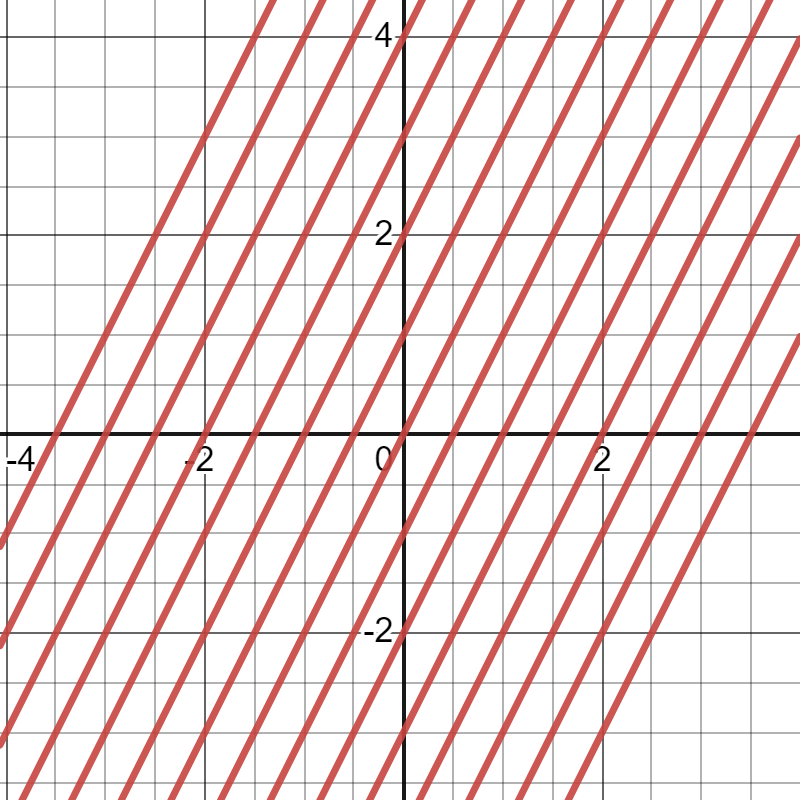
\includegraphics[scale=0.15]{desmos-graph.png}\\
                 $$y=c_2$$
             \centering
                 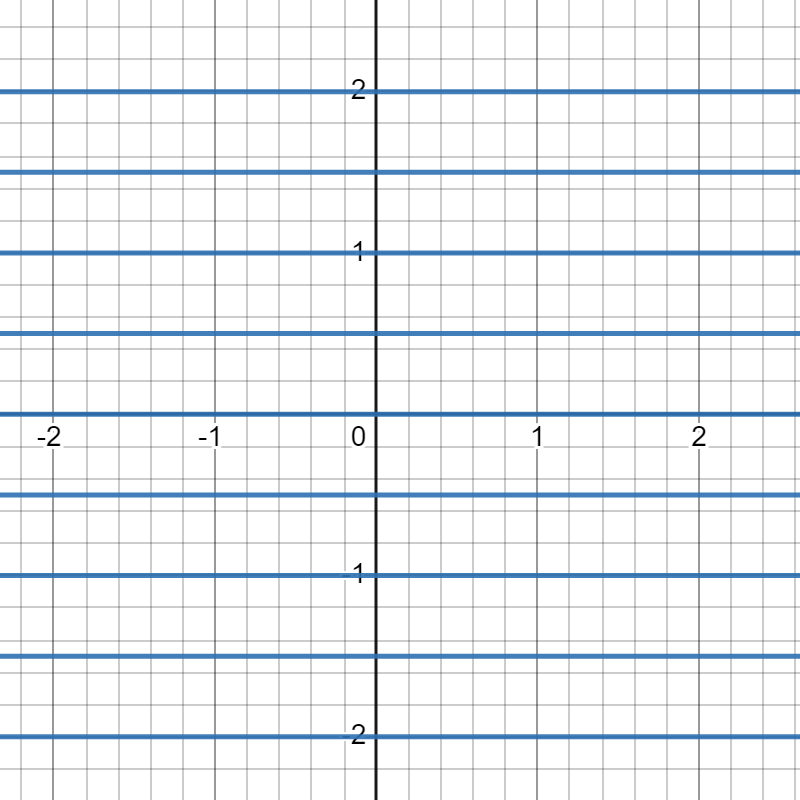
\includegraphics[scale=0.15]{desmos-graph (1).png}
                
           
              
               
            \qed
        \end{solucion}
    \end{itemize}
\end{homeworkProblem}

\newpage

\begin{homeworkProblem}
    Considere la ecuación
    $$u_{xx}+4u_{xy}+u_x=0$$
    \begin{itemize}
        \item [i)] Lleve la ecuación a la forma canónica.
        \begin{solucion}
         Los coeficientes de la ecuación son $a=1, b=2$ y $c=0$ luego el discriminante es:
         $$\delta(x,y)=2^2-1\cdot0=4>0$$
         Por lo tanto la ecuación es \textbf{hiperbólica} y podemos determinar los cambios de variable gracias a las características:
         $$\dfrac{dy}{dx}=2\pm2$$
         Luego solucionando y despejando para constantes tenemos que:
         \begin{align*}
             y&=4x+c_1 & y&=c_2\\
             c_1&=y-4x
         \end{align*}
         Luego si tomamos a $\xi=c-1$ y $\eta=c_2$ tenemos nuestros cambios de variables $\xi=y-4x$ y $\eta=y$. Determinemos las derivadas necesarias para llevar la EDP a la forma canónica considerando $V(\xi,\eta)=u(x,y)$:
         \begin{align*}
          u_x&=V_\xi\xi_x+V_\eta\eta_x\\
          &=-4V_\xi\\
          \\
          u_{xx}&=-4(V_{\xi\xi}\xi_x+V_{\xi\eta}\eta_x)\\
          &=16V_{\xi\xi}\\
          \\
          u_{xy}&=-4(V_{\xi\xi}\xi_y+V_{\xi\eta}\eta_y)\\
          &=-4V_{\xi\xi}-4V_{\xi\eta}
         \end{align*}
         y reemplazando obtenemos que:
         \begin{align*}
          u_{xx}+4u_{xy}+u_x&=16V_{\xi\xi}+4(-4V_{\xi\xi}-4V_{\xi\eta})-4V_\xi\\
          &=-16V_{\xi\eta}-4V_\xi
         \end{align*}
         Así tenemos que:
         $$-16V_{\xi\eta}=4V_\xi$$
         y simplificando llegamos a que la forma canónica de la EDP es:
         $$V_{\xi\eta}=-\dfrac{1}{4}V_\xi$$
         \qed
        \end{solucion}
        \item [ii)] Encuentre la solución especifica $u(x,8x)=0,u_x(x,8x)=4e^{-2x}.$
        \begin{solucion}
           Si realizamos la sustitución $w=V_\xi$ en la forma canónica obtenida tenemos que:
           $$ \dfrac{\partial w}{\partial\eta}=-\dfrac{1}{4}w$$
           De esta forma la EDP no depende $\xi$ y podemos buscar solución como si fuera una EDO por medio de la separación de variables:
           \begin{align*}
               \int\dfrac{\partial w}{w}&=-\dfrac{1}{4}\int\partial\eta\\
               \log w&=-\dfrac{1}{4}\eta+c(\xi)\\
               w&=g(\xi)e^{-\frac{1}{4}\eta}
           \end{align*}
           Ahora devolvamos nuestra sustitución y resolvamos nuevamente simplemente integrando en ambos lados de la ecuación respecto a $\xi$:
           \begin{align*}
               V_\xi=w&=g(\xi)e^{-\frac{1}{4}\eta}\\
               \int V_\xi\,d\xi&=e^{-\frac{1}{4}\eta}\int g(\xi)\,d\xi\\
               V&=e^{-\frac{1}{4}\eta}G(\xi)+C(\eta)
           \end{align*}
           Aquí como $g(\xi)$ es una función de una sola variable suponemos que la integramos normalmente y nos genera otra función de una variable $G(\xi)$ mas una función que depende de $\eta$ ya que al realizar la derivada parcial respecto a $\xi$ esa se haría 0. Recordemos que $V(\xi,\eta)=u(x,y)$ y que nuestro cambio de variable estaba dado por $\xi=y-4x$ y $\eta=y$ así que podemos expresar nuestra solución general en términos de $x$ y $y$ y quedaría:
           $$u(x,y)=e^{-\frac{1}{4}y}G(y-4x)+C(y)$$
           De esta manera podemos usar nuestras condiciones iniciales para hallar la solución especifica:
           \begin{align*}
               0&=u(x,8x)=e^{-2x}G(4x)+C(8x)\\
               4e^{-2x}&=u_x(x,8x)=e^{-2x}(-4G^\prime(4x))
           \end{align*}
           De segunda ecuación despejando para $G^\prime$ obtenemos que:
           $$G^\prime(4x)=-1$$
           e integrando a ambos lados respecto a $x$ obtenemos que:
           $$G(4x)=-4x$$
           Ahora reemplazando este valor en la primera ecuación y despejando para $C$ obtenemos que
           $$C(8x)=4xe^{-2x}$$
           Ahora recordemos que nosotros queremos hallar quienes son $C(y)$ y $G(y-4x)$ pero notemos que:
           \begin{align*}
               C(y)&=C\left(8\left(\frac{y}{8}\right)\right)=\dfrac{y}{2}e^{-\frac{1}{4}y}\\
               \\
               G(y-4x)&=G\left(4\left(\frac{y}{4}-x\right)\right)=-4\left(\frac{y}{4}-x\right)=-y+4x
           \end{align*}
           y reemplazando en nuestra solución general obtenemos que la solución especifica es:
           $$u(x,y)=e^{-\frac{1}{4}y}(-y+4x)+\frac{y}{2}e^{-\frac{1}{4}y}=4xe^{-\frac{1}{4}y}-\dfrac{y}{2}e^{-\frac{1}{4}y}$$
           Aunque solo por seguridad verifiquemos si esta solución satisface la EDP original y cumple las condiciones iniciales:
           \begin{align*}
               u_x(x,y)&=4e^{-\frac{1}{4}y}\\
               \\
               u_{xx}(x,y)&=0\\
               \\
               u_{xy}(x,y)&=-e^{-\frac{1}{4}y}         
           \end{align*}
            Con esta información reemplacemos y veamos que si da $0$:
            \begin{align*}
                u_{xx}+4u_{xy}+u_x&=0+4(-e^{-\frac{1}{4}y})+4e^{-\frac{1}{4}y}\\
                    &=0
            \end{align*}
            Ahora que confirmamos que satisface la EDP veamos que si satisface las condiciones iniciales:
            \begin{align*}
                u(x,8x)&=4xe^{-\frac{1}{4}(8x)}-\dfrac{8x}{2}e^{-\frac{1}{4}(8x)}\\
                        &=4xe^{-2x}-4xe^{-2x}\\
                        &=0\\
                        \\
                u_x(x,8x)&=4e^{-\frac{1}{4}(8x)}\\
                &=4e^{-2x}       
            \end{align*}
           Como cumple la EDP y las condiciones iniciales ahora si con toda seguridad podemos decir que es la solución especifica.
           \qed
        \end{solucion}
    \end{itemize}
\end{homeworkProblem}
\newpage
\begin{homeworkProblem}
Sea $U \subset \mathbb{R}^2$ un abierto. Considere la ecuación de segundo orden
$$
a(x, y) \frac{\partial^2 u}{\partial x^2}+2 b(x, y) \frac{\partial^2 u}{\partial x \partial y}+c(x, y) \frac{\partial^2 u}{\partial y^2} u=0
$$
donde $u: U \rightarrow \mathbb{R}$ pertenece $C^2(U)$ y los términos $a, b, c$ son funciones $C^1(U)$. Definimos el discriminante de la EDP por
$$
\delta(x, y)=b^2(x, y)-a(x, y) c(x, y) .
$$

Considere el cambio de variable
$$
\xi=\xi(x, y), \quad \eta=\eta(x, y)
$$
donde las funciones son de clase $C^2(U)$ y el Jacobiano $\operatorname{det}\left(\frac{\partial(\xi, \eta)}{\partial(x, y)}\right) \neq 0$ en todo punto $(x, y) \in U$.\\
\\
    Muestre que el signo del discriminante $\delta(x, y)$ es invariante por el cambio de variables $(\xi, \eta)$. Es decir, considere $v(\xi, \eta)=u(x, y)$, usando que u satisface la EDP original, muestre que $v$ satisface la ecuación:
$$
A(\xi, \eta) \frac{\partial^2 v}{\partial \xi^2}+2 B(\xi, \eta) \frac{\partial^2 v}{\partial \xi \partial \eta}+C(\xi, \eta) \frac{\partial^2 v}{\partial \eta^2}=G\left(\xi, \eta, \nu, \frac{\partial v}{\partial \xi}, \frac{\partial v}{\partial \eta}\right),
$$
para algunas funciones $A, B, C, G$. Luego muestre que el signo de $\delta(\xi, \eta)=B^2(\xi, \eta)-$ $A(\xi, \eta) C(\xi, \eta)$ es igual al signo de $\delta(x, y)$.
    \begin{solucion}
        Por simpleza de ahora en adelante escribiremos $a=a(x,y),b=b(x,y)$ y $c=c(x,y)$ entonces nuestra EDP reescrita queda como:
        $$au_{xx}+2bu_{xy}+cu_{yy}=0$$
        Ahora por el cambio de variable $\xi=\xi(x,y)$ y $\eta=\eta(x,y)$ como estas funciones son $C^2(U)$ por hipótesis podemos derivar sin ningún problema. Si consideramos $V(\xi,\eta)=u(x,y)$ tenemos que:
        \begin{align*}
            u_x&=V_\xi\xi_x+V_\eta\eta_x\\
            \\
            u_{xx}&=(V_{\xi\xi}\xi_x+V_{\xi\eta}\eta_x)\xi_x+V_\xi\xi_{xx}+(V_{\eta\eta}\eta_x+V_{\xi\eta}\xi_x)\eta_x+V_\eta\eta_{xx}\\
            &=\xi^2_xV_{\xi\xi}+2\xi_x\eta_xV_{\xi\eta}+\eta^2_xV_{\eta\eta}+V_\xi\xi_{xx}+V_\eta\eta_{xx}\\
            \\
            u_{xy}&=(V_{\xi\xi}\xi_y+V_{\xi\eta}\eta_y)\xi_x+V_\xi\xi_{xy}+(V_{\eta\eta}\eta_y+V_{\xi\eta}\xi_y)\eta_x+V_\eta\eta_{xy}\\
            &=\xi_x\xi_yV_{\xi\xi}+(\xi_x\eta_y+\xi_y\eta_x)V_{\xi\eta}+\eta_x\eta_yV_{\eta\eta}+V_\xi\xi_{xy}+V_\eta\eta_{xy}\\
            \\
            u_y&=V_\xi\xi_y+V_\eta\eta_y\\
            \\
            u_{yy}&=(V_{\xi\xi}\xi_y+V_{\xi\eta}\eta_y)\xi_y+V_\xi\xi_{yy}+(V_{\eta\eta}\eta_y+V_{\xi\eta}\xi_y)\eta_y+V_\eta\eta_{yy}\\
            &=\xi^2_yV_{\xi\xi}+2\xi_y\eta_yV_{\xi\eta}+\eta^2_yV_{\eta\eta}+V_\xi\xi_{yy}+V_\eta\eta_{yy}\\
        \end{align*}
        Con todo esto si reemplazamos en la EDP original ya que $u(x,y)$ la satisface tenemos la siguiente EDP:
        \begin{multline*}
            a\xi^2_xV_{\xi\xi}+2a\xi_x\eta_xV_{\xi\eta}+a\eta^2_xV_{\eta\eta}+aV_\xi\xi_{xx}+aV_\eta\eta_{xx}\\
         +2b\xi_x\xi_yV_{\xi\xi}+2b(\xi_x\eta_y+\xi_y\eta_x)V_{\xi\eta}+2b\eta_x\eta_yV_{\eta\eta}+2bV_\xi\xi_{xy}+2bV_\eta\eta_{xy}\\
        +c\xi^2_yV_{\xi\xi}+2c\xi_y\eta_yV_{\xi\eta}+c\eta^2_yV_{\eta\eta}+cV_\xi\xi_{yy}+cV_\eta\eta_{yy}=0
        \end{multline*}
        Si juntamos términos semejantes y dejamos los términos de orden menor al lado derecho de la ecuación tenemos que:
        \begin{multline*}
            (a\xi_x^2+2b\xi_x\xi_y+c\xi_y^2)V_{\xi\xi}
            +2(a\xi_x\eta_x+b\xi_x\eta_y+b\xi_y\eta_x+c\xi_y\eta_y)V_{\xi\eta}
            +(a\eta_x^2+2b\eta_x\eta_y+c\eta_y^2)V_{\eta\eta}\\
            =-\left[(a\xi_{xx}+2b\xi_{xy}+c\xi_{yy})V_\xi+(a\eta_{xx}+2b\eta_{xy}+c\eta_{yy})V_\eta\right]
        \end{multline*}
        Por hipótesis $J=\det\left(\dfrac{\partial(\xi,\eta)}{\partial(x,y)}\right)=\xi_x\eta_y-\xi_y\eta_x\neq0$ en todo $(x,y)\in U$, es decir nuestro cambio de variable es invertible y todas las funciones que dependen de $x$ y $y$ se pueden reescribir en términos de $\xi$ y $\eta$, así mismo  las derivadas de $\xi$ y $\eta$ respecto a $x$ y $y$ se pueden reescribir solo en términos de $\xi$ y $\eta$. Así podemos concluir que $V$ satisface:
        $$A(\xi,\eta)V_{\xi\xi}+2B(\xi,\eta)V_{\xi\eta}+C(\xi,\eta)V_{\eta\eta}=G(\xi,\eta,V,V_\xi,V_\eta)$$

        Donde tenemos que:
        \begin{align*}
           A=A(\xi,\eta)&=a\xi_x^2+2b\xi_x\xi_y+c\xi_y^2\\
           B=B(\xi,\eta)&=a\xi_x\eta_x+b\xi_x\eta_y+b\xi_y\eta_x+c\xi_y\eta_y\\
           C=C(\xi,\eta)&=a\eta_x^2+2b\eta_x\eta_y+c\eta_y^2\\
           G=G(\xi,\eta,V,V_\xi,V_\eta)&=-\left[(a\xi_{xx}+2b\xi_{xy}+c\xi_{yy})V_\xi+(a\eta_{xx}+2b\eta_{xy}+c\eta_{yy})V_\eta\right]
        \end{align*}

        Ya con esto recordemos que el discriminante del original esta dado por:
        $$\delta(x,y)=b^2-ab$$
        Ahora tenemos una nueva EDP y su discriminante esta dado por:
        $$\delta(\xi,\eta)=B^2-AC$$
        Ahora calculemos estaos valores para determinar si hay alguna relación entre los dos discriminantes:
        \begin{multline*}
            B^2=a^2\xi_x^2\eta_x^2+b^2\xi_x^2\eta_y^2+b^2\xi_y^2\eta_x^2+c^2\xi_y^2\eta_y^2+2ab\xi_x^2\eta_x\eta_y+2ab\xi_x\xi_y\eta_x^2+2ac\xi_x\xi_y\eta_x\eta_y\\
            +2b^2\xi_x\xi_y\eta_x\eta_y+2bc\xi_x\xi_y\eta_y^2+2bc\xi_y^2\eta_x\eta_y
            \end{multline*}
            \begin{multline*}
                AC=a^2\xi_x^2\eta_x^2+2ab\xi_x^2\eta_x\eta_y+ac\xi_x^2\eta_y^2+2ab\xi_x\xi_y\eta_x^2+4b^2\xi_x\xi_y\eta_x\eta_y+2bc\xi_x\xi_y\eta_y^2\\
                +ac\xi_y^2\eta_x^2+2bc\xi_y^2\eta_x\eta_y+c^2\xi_y^2\eta_y^2
            \end{multline*}
            Así entonces tenemos que:
            \begin{align*}
                B^2-AC&=b^2\xi^2\eta_y^2+b^2\xi_y^2\eta_x^2+2ac\xi_x\xi_y\eta_x\eta_y+2b^2\xi_x\xi_y\eta_x\eta_y-ac\xi_x^2\eta_y^2-4b^2\xi_x\xi_y\eta_x\eta_y-ac\xi_y^2\eta_x^2\\
                &=(b^2-ac)\xi_x^2\eta_y^2+(b^2-ac)\xi_y^2\eta_x^2-2(b^2-ac)\xi_x\xi_y\eta_x\eta_y\\
                &=(b^2-ac)(\xi_x^2\eta_y^2-2\xi_x\xi_y\eta_x\eta_y+\xi_y^2\eta_x^2)\\
                &=(b^2-ac)(\xi_x\eta_y-\xi_y\eta_x)^2
            \end{align*}
            Ahora del lado izquierdo tenemos el discriminante de nuestra EDP luego del cambio de variable y al lado derecho tenemos el discriminante de la EDP original multiplicada por el jacobiano al cuadrado, es decir podemos reescribir esta expresión como: 
            $$\delta(\xi,\eta)=\delta(x,y)J^2$$
            Ahora como por hipótesis $J\neq0$ tenemos que $J^2>0$ por lo que este no afectara el signo del discriminante nuevo. Siendo mas explícitos esta expresión nos dice que si $\delta(x,y)>0$ entonces $\delta(\xi,\eta)>0$, si $\delta(x,y)=0$ entonces $\delta(\xi,\eta)=0$ y si $\delta(x,y)<0$ entonces $\delta(\xi,\eta)<0$, es decir que independientemente del cambio de variable ya que propusimos uno arbitrario que cumpla las condiciones iniciales tenemos que el discriminaste no cambia su signo, o en otras palabras el discriminante es invariante por el cambio de variables. 
            \qed
    \end{solucion}
\end{homeworkProblem}
%%%%%%%%%%%%%%%%%%%%%%%%%%%%%%%%%%%%%%%%%%%%%%%%%%%%%%%
\end{document}